\problemname{}

%\illustration{0.3}{image.jpg}{
%    Caption of the illustration (optional).
%    CC BY-SA 4.0 by X on \href{https://example.com/reference-to-image}{Y}
%}

A sliding puzzle consists of square tiles on a rectangular grid.
Exactly one of the grid positions is empty, so that you can move
the tile above, below, to its left, or to its right
into the empty square and back.

Each tile is labelled with a unique number,
as shown in Figure~\ref{fig:puzzle}.
To solve a sliding puzzle,
you need to find a sequence of moves that puts the tile numbers
in ascending order, from left to right and top to bottom,
such that the empty square ends up at the bottom right position in the grid,
as shown in Figure~\ref{fig:solved}.
Such a sequence of moves does not exist for all sliding puzzles.

\begin{figure}[!h]
  \begin{minipage}[t]{.3\textwidth}
    \centering
    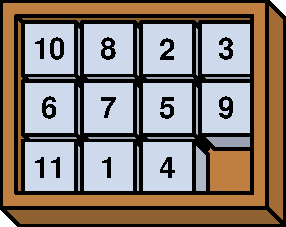
\includegraphics[width=\textwidth]{puzzle.pdf}
    \ifcsname captionsetup\endcsname
    \captionsetup{width=\textwidth}
    \fi
    \caption{Example of a 3-by-4 sliding puzzle, corresponding to Sample Input 1.}
    \label{fig:puzzle}
  \end{minipage}
  \hfill
  \begin{minipage}[t]{.3\textwidth}
    \centering
    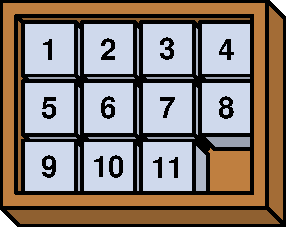
\includegraphics[width=\textwidth]{solvedpuzzle.pdf}
    \ifcsname captionsetup\endcsname
    \captionsetup{width=\textwidth}
    \fi
    \caption{The sliding puzzle of Figure~\ref{fig:puzzle} after solving.}
    \label{fig:solved}
  \end{minipage}
  \hfill
  \begin{minipage}[t]{.3\textwidth}
    \centering
    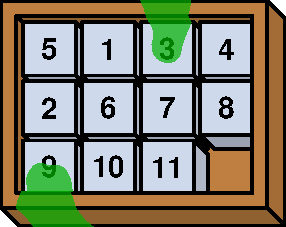
\includegraphics[width=\textwidth]{gluedpossible.pdf}
    \ifcsname captionsetup\endcsname
    \captionsetup{width=\textwidth}
    \fi
    \caption{Example of a sliding puzzle with glued tiles,
             covered in green goo.
             This example is possible to solve, corresponding to Sample Input 3.}
    \label{fig:gluedpossible}
  \end{minipage}
\end{figure}

While cleaning out your garage,
you grapple with the garage goblins over a glowing box full of goodies.
They offer a gamble:
the box is yours if you can solve all their sliding puzzles.
You accept to give it a go,
only to find out that the garage goblins have glued some tiles in place!
The glued tiles no longer move, as shown in Figure~\ref{fig:gluedpossible}.

However, all sliding puzzles share the following properties:
\begin{itemize}
\item The empty square is at the bottom right position.
\item Every glued tile is in its correct position.
\item For each tile that can move, there is a sequence of moves
  that leaves the empty square in its position instead.
\item From any glued tile,
  there is a path to the border of the sliding puzzle across glued tiles only,
  when stepping to the tile above, below, to the left, or to the right at each step.
  That is, no glued tiles are encircled by tiles that can move.
\end{itemize}

Determine whether it is possible to solve a given sliding puzzle.

\begin{Input}
  The input consists of:
  \begin{itemize}
    \item One line with two integers $h$ and $w$ ($1 \le h,w \le 500$), the
      height and width of the sliding puzzle's grid.
    \item $h$ lines with $w$ characters,
      each character being either `\texttt{.}'\ or `\texttt{\#}'.
      The bottom right character, at the position of the empty square,
      is `\texttt{.}'.
      Otherwise, `\texttt{.}'\ denotes a tile that can move,
      and `\texttt{\#}' denotes a glued tile.
    \item $h$ lines with $w$ integers $a_{i,j}$
      ($1 \le i \le h$, $1 \le j \le w$, $0 \le a_{i,j} \le h \cdot w - 1$).
      The bottom right integer is $a_{h,w} = 0$, representing the empty square.
      Otherwise, $a_{i,j}$ is the label on the tile at position $(i,j)$.
  \end{itemize}
  The set of all $a_{i,j}$ ($1 \le i \le h, 1 \le j \le w$)
  contains each of the numbers $0, 1, \dots, h \cdot w - 1$ once.
\end{Input}

\begin{Output}
  Output \texttt{possible} if the sliding puzzle can be solved, or
  \texttt{impossible} if not.
\end{Output}
